\documentclass[11pt]{report}
\usepackage{outline}
\usepackage{pmgraph}
\usepackage[normalem]{ulem}
\usepackage[utf8]{inputenc}
\usepackage[T1]{fontenc}
\usepackage[french]{babel}
\title{\textbf{GIF-4100 : Vision numérique\\ Projet de trimestre \\La feuille électronique}}
\author{Olivier Beaulieu,\\Frédéric Bernard,\\Kento Otomo-Lauzon}
%% \date{\oldstylenums{00}/\oldstylenums{00}/\oldstylenums{00}}
%--------------------Make usable space all of page
\setlength{\oddsidemargin}{0in}
\setlength{\evensidemargin}{0in}
\setlength{\topmargin}{0in}
\setlength{\headsep}{-.25in}
\setlength{\textwidth}{6.5in}
\setlength{\textheight}{8.5in}
%--------------------Indention
\setlength{\parindent}{1cm}
\usepackage{graphicx}
\graphicspath{ {assets/} }

\begin{document}
%--------------------Title Page
\maketitle
 

\newpage

\section{Solution proposée}
La solution proposée est constituée d'un projecteur et d'une caméra. Le
projecteur est disposé de manière à illuminer une table, et la caméra sert à
détecter la position de feuilles blanches et d'un doigt.

\subsection{Fonctionnement général}
Le système permet à un utilisateur, en utilisant son doigt, de dessiner sur une
feuille en temps réel. En localisant la position du doigt et de la feuille
blanche sur la table, le système superpose le tracé effectué par l'utilisateur
sur la feuille. Dans le cas où plusieurs feuilles sont présentes sur la table,
le dessin est dupliqué sur chaque feuille. Le dessin étant défini de manière
relative à la feuille, celui-ci demeure à l'endroit, et ce, même si
l'utilisateur déplace la feuille ou lui fait effectuer une rotation.

Finalement, le dessin est visible depuis une application web, laquelle est
accessible depuis un ordinateur.

Dans un contexte de télétravail, on pourrait imaginer un scénario d'utilisation
selon lequel deux collègues sont disposés autour de la table en ayant chacun une
feuille. Les membres physiquement présents à la réunion pourraient participer à
une séance de remue-méninges en dessinant sur leur propre feuille, et le
résultat serait automatiquement reflété sur les feuilles des autres
participants. De plus, des participants présents à distance pourraient effectuer
le même exercice en se connectant à l'application web. 

\subsection{Description de la méthode employée}
Cette section décrit les aspects techniques nécessaires à la réalisation du
projet. L'application des algorithmes de vision artificielle est faite à l'aide
de la bibliothèque \textit{OpenCV}, l'affichage graphique pour le projecteur est
faite au moyen du module \textit{Python} \textit{Tkinter}, l'application web est
faite avec \textit{VueJS} et la gestion du serveur et du flot d'exécution est
faite par le \textit{framework} \textit{Jivago}. 

\subsubsection{Détection de la feuille blanche}
La figure \ref{feuille_blanche} montre une vue qu'aurait la caméra du la surface
de travail. Les paramètres de saisie de la caméra ont été choisis de sorte à
faire ressortir la surface blanche sous l'éclairage dominant du projecteur. Par
la suite, un seuillage sur les valeurs d'illuminance est effectué, de sorte à ne
conserver que les pixels dont la « valeur » dans le repère HSV est supérieure à
150, et ce, peu importe la valeur de \textit{hue} ou de \textit{saturation}.

Ensuite, on identifie le rectangle englobant d'aire minimale pour obtenir
l'orientation de la feuille et la coordonnée des coins, dans le repère caméra.
Un exemple de détection est présenté à la figure \ref{detection_feuille}.

\begin{figure}[h]
  \centering
  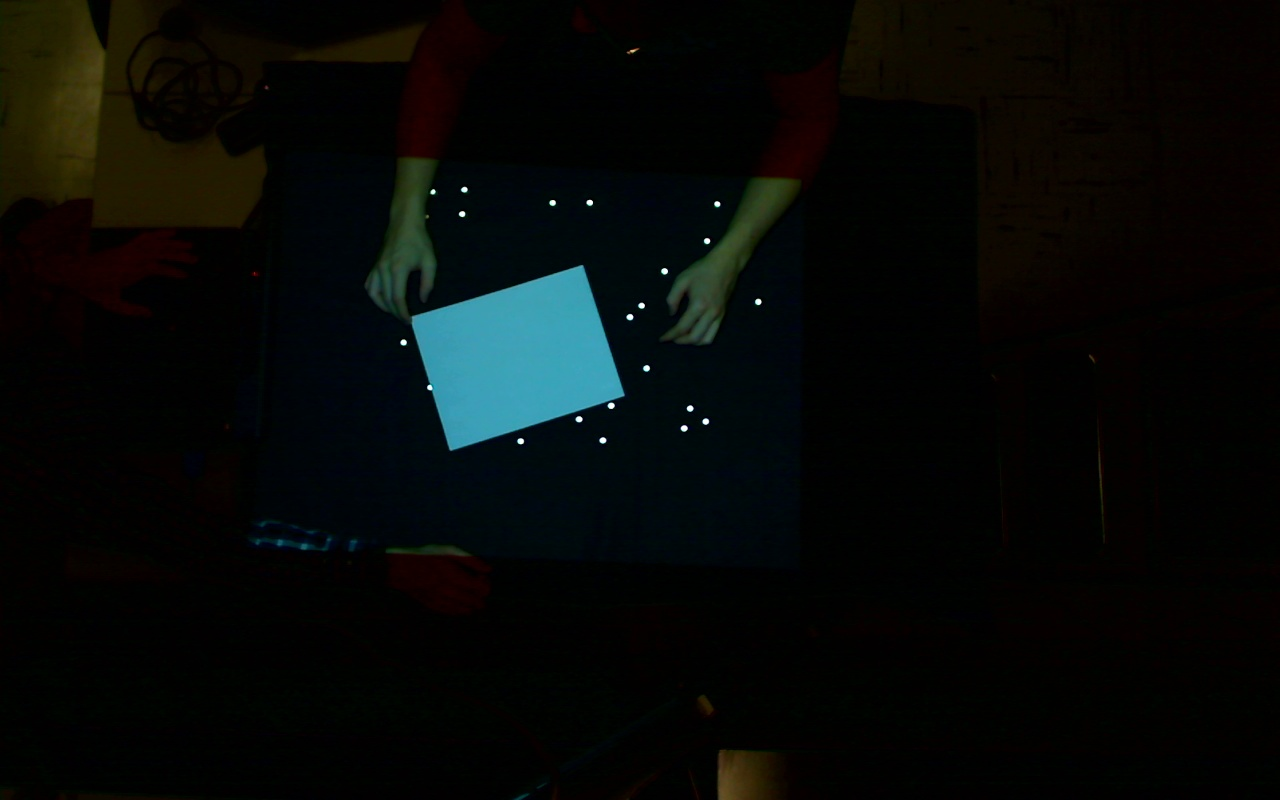
\includegraphics[width=8cm]{feuille-blanche.jpg}
  \caption{Vue de la caméra}
  \label{feuille_blanche}
\end{figure}

\begin{figure}[h]
  \centering
  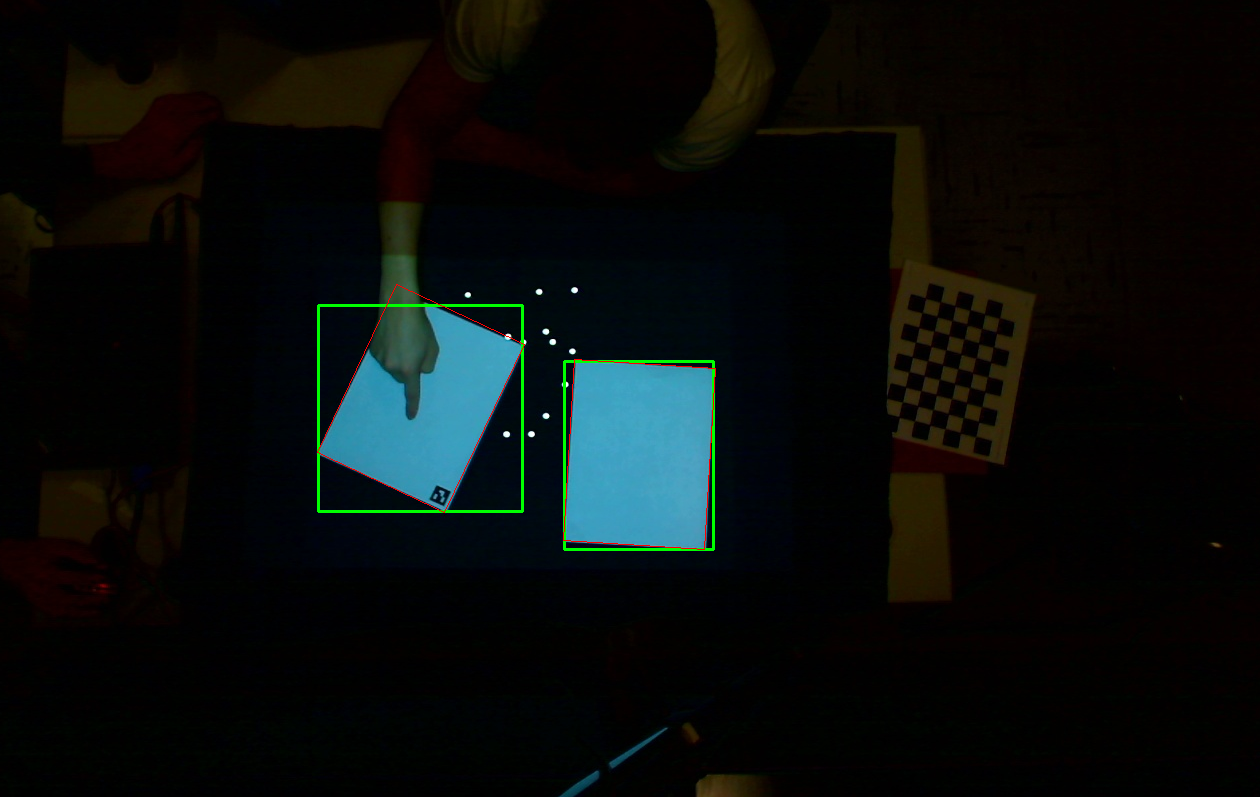
\includegraphics[width=8cm]{localisation-feuille.png}
  \caption{Délimitation des feuilles blanches.
    Le rectangle rouge correspond au rectangle englobant d'aire minimale.}
  \label{detection_feuille}
\end{figure}

\subsubsection{Détection du doigt}
Similairement, la détection du doigt s'effectue par un seuillage appliqué sur la
valeur HSV des pixels. Pour le moment, un seuil est prédéfini de manière à
reconnaître la main de l'un des présentateurs. La position du doigt elle-même
est choisie comme le point les plus éloigné du centre de masse de l'amas de
pixels représentant le bras de l'expérimentateur. La figure
\ref{detection_doigt} illustre le résultat de cette procédure.

\begin{figure}[h]
  \centering
  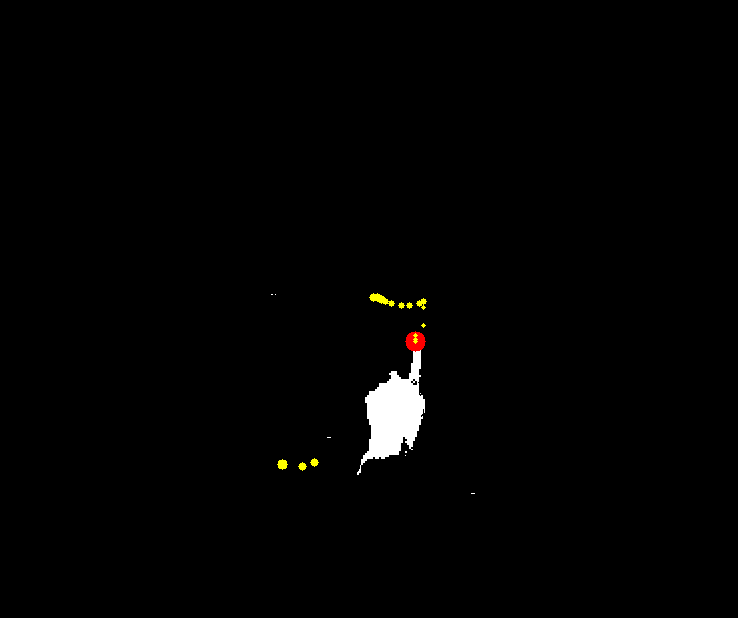
\includegraphics[width=8cm]{detection-doigt.png}
  \caption{Filtre appliqué pour détecter le doigt. Le point rouge correspond à
    la position identifiée pour le doigt, et les points jaunes correspondent aux
    positions passées.}
  \label{detection_doigt}
\end{figure}


\subsubsection{Homographie entre l'image projetée et l'image capturée par la
  caméra}
La calibration initiale de la caméra est effectuée au moyen d'un damier. De
cette manière, nous sommes en mesure d'annuler les effets de la distorsion sur
les images captées.

Afin d'effectuer la conversion des coordonnées entre les repères de la caméra et
du projecteur, l'appariement initial des points pour le calcul de l'homographie
est effectué au moyen d'un marqueur \textit{ArUco}. Avant de débuter la
démonstration, le script de calibration est lancé, et projette un marqueur.
L'appariement des quatre coins est effectué en utilisant les algorithmes de
détection d'\textit{ArUco} disponibles dans \textit{OpenCV}. 

% TODO : image processus de calibrataion

\subsubsection{Logique de gestion de dessin}

Le dessin à afficher est sauvegardé de manière vectorielle. Chaque ligne est
enregistrée individuellement, et les distances sont encodées en millimètres, et
sont calculées en utilisant la définition du format de papier \textit{US
  Letter} (8.5po x 11po). Cette gestion permet de maintenir la taille du dessin,
dans le cas où la feuille est placée plus ou moins loin du projecteur.

Un \textit{thread} en arrière plan se charge de maintenir à jour le canevas qui
est projeté, de sorte que l'affiche s'effectue en temps réel. 

\subsubsection{Application web de visualisation et d'administration}

Enfin, plusieurs routes d'API REST sont exposées au moyen d'une application
\textit{Jivago}, ce qui permet à une application web de visualiser en direct le
dessin. L'application web elle-même, récupère l'information du canevas à chaque
seconde pour l'afficher (figure \ref{web_ui}). 

\begin{figure}
  \centering
  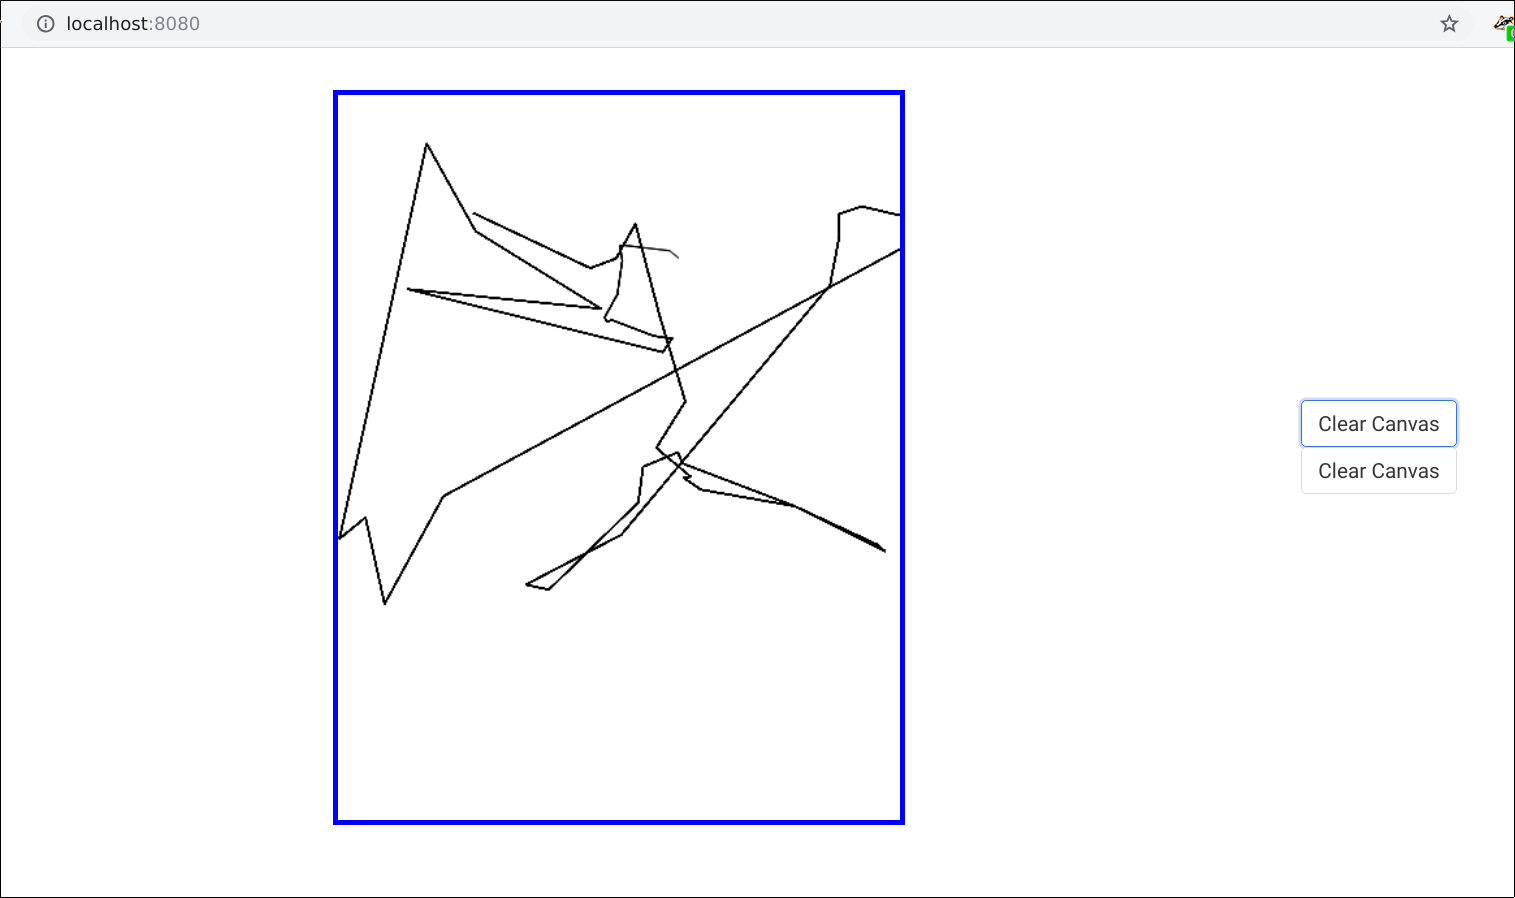
\includegraphics[width=8cm]{web-canvas.png}
  \caption{Affichage du canevas en direct depuis un navigateur web.}
  \label{web_ui}
  \end{figure}

\section{Performances}

\section{Améliorations possibles}
% Utiliser une seconde caméra pour identifier quand on touche vs quand on touche pas
% Faire un « calibrage » sur le seuillage de couleur pour trouver le bras




\end{document}
